\documentclass[../main.tex]{subfiles}
\begin{document}


\subsection{Creazione Macchina}
Come prima cosa bisognerà aprire virtual box e cliccare in alto a destra sul tasto \textbf{Nuova} una volta fatto ci si aprirà la seguente schermata. In questa schermata andrà scelto il nome della macchina, dove salvare e in fine che sistema operativo vogliamo installare. 


\begin{figure}[h]
    \centering
    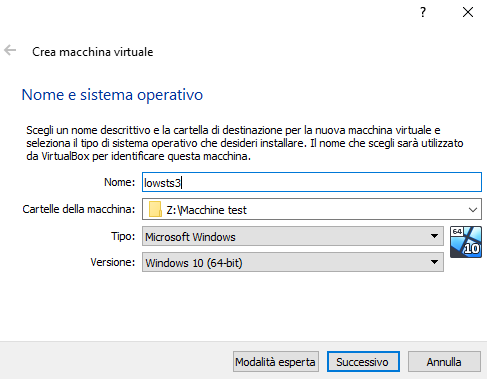
\includegraphics[width=0.6\textwidth]{Images/set-up1.PNG}
    \caption{Nome macchina}
\end{figure}
  Una votla fatto questo ci basterà cliccare su \textbf{Successivo} per andare avanti con l'installazione. E verremo portati alla schermata seguent.
  
\

\begin{figure}[h]
    \centering
    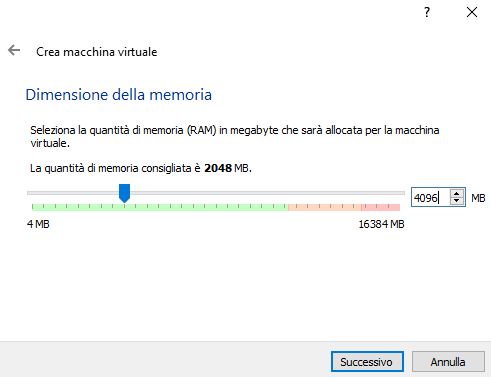
\includegraphics[width=0.6\textwidth]{Images/set-up2.PNG}
    \caption{Assegnazione RAM}
\end{figure}

\pagebreak{}
\thispagestyle{header-pages}

Una votla arrivati in questa schermata dovremmo solo impostare la ram in questo caso avendo a disposizione una macchina con 16 GB di RAM ho deciso di dare 4 GB di RAM a questa macchina virtuale. Anche qui una volta imessa quanta RAM vogliamo ci basterÀ cliccare successivo e procedere.

\textbf{Remember la quantità di RAM che assegni deve essere 1024 moltipilicato quanta ram vuoi dare nel mio caso 4GB di RAM quindi 1024*4}

Per le prossime due schermata ci basterà andare avanti. Fino a arrivare alla schermata seguente

\begin{figure}[h]
    \centering
    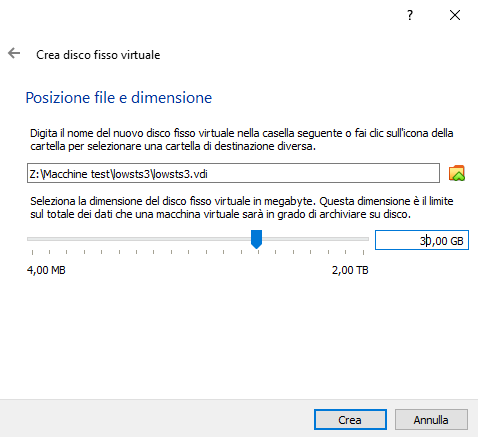
\includegraphics[width=0.5\textwidth]{Images/set-up5.PNG}
    \caption{Assegnazione spazio al disco}
\end{figure}

In questa schermata dovremmo insteire quanta memoria vorrrmo che la nostra macchina virtuale abbia in questo caso scriviamo 30,00 GB e cliccare il tasto \textbf{Crea}.


\begin{figure}[h]
    \centering
    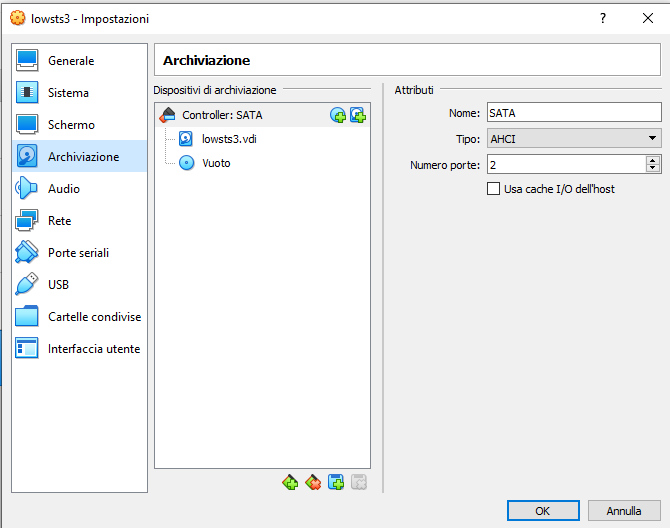
\includegraphics[width=0.5\textwidth]{Images/set-up6.PNG}
    \caption{Aggiunta dell'ISO}
\end{figure}
\pagebreak{}
\thispagestyle{header-pages}


Una volta fatto tutto questo ci manca solo l'ultima cosa cioè collegare la iso alla nostra macchina virtuale. Ci basterà cliccare sul disco vuoto e cliccare aggiungi e selezionare la nostra iso.


Una volta fatto questo dovremmo modificare anche le schede di rete, dove troveremo già attiva sulla scheda di rete 1 il NAT e nella scheda di rete due dovremmo abilitare la rete interna. 

\begin{figure}[h]
    \centering
    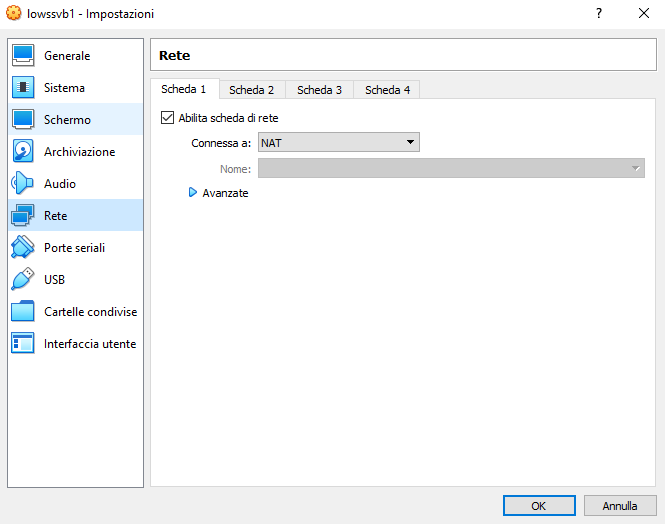
\includegraphics[width=0.75\textwidth]{Images/set-up7.PNG}
    \caption{Internet}
\end{figure}

Una volta avviata la macchina virtuale partirà questa schermata ci basterà cliccare \textbf{next}e poi \textbf{installa}.

\begin{figure}[h]
    \centering
    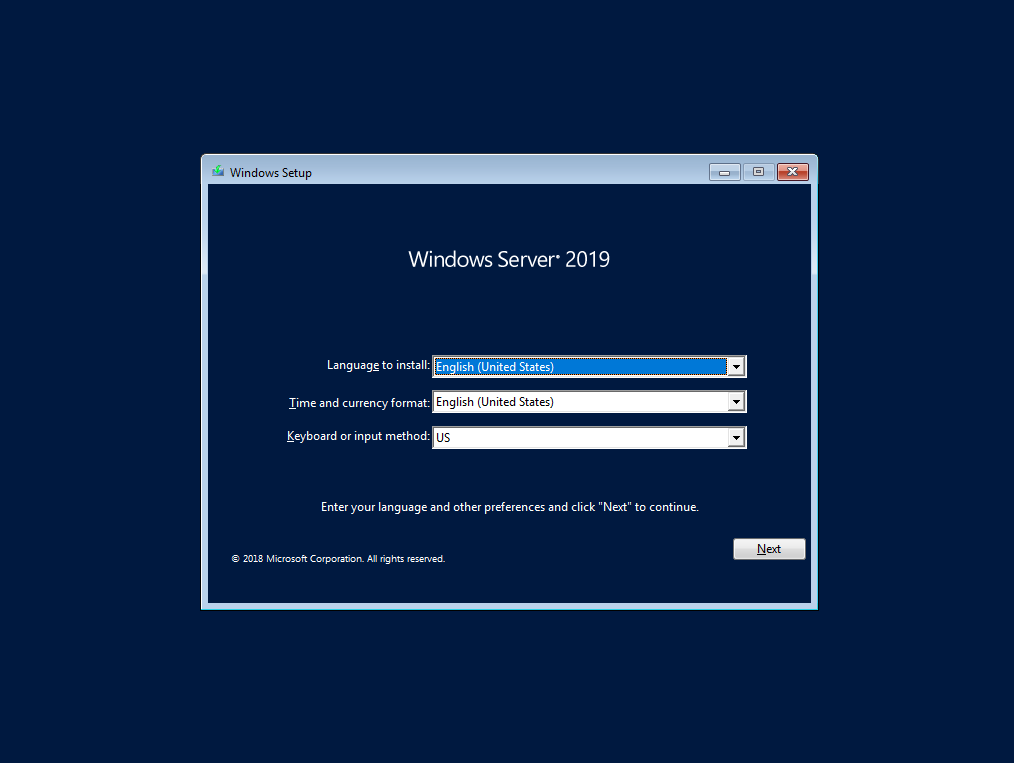
\includegraphics[width=0.5\textwidth]{Images/conf1en.PNG}
    \caption{Aggiunta dell'ISO}
\end{figure}

\pagebreak{}
\thispagestyle{header-pages}

\subsubsection{Versione Core}
Qui ci basterà cliccare la versione nel nostro caso Windows Server 2019 Standard Evaluation e cliccare su \textbf{next}.Dopo di che ci chiederà di accettare i termini della licenza bisogna accettare e andare avanti. Ci caricherà una schermata dove che tipo di installazione si vuole eseguire. Noi sceglieremo Quella personalizzata, ci verrà chiesto su che disco la vogliamo installare e ci mostrerà solo un disco. Quindi senza fare niente ci basterà cliccare su \textbf{next}. Dopo aver cliccato avanti partirà l'installazione. 

\begin{figure}[h]
    \centering
    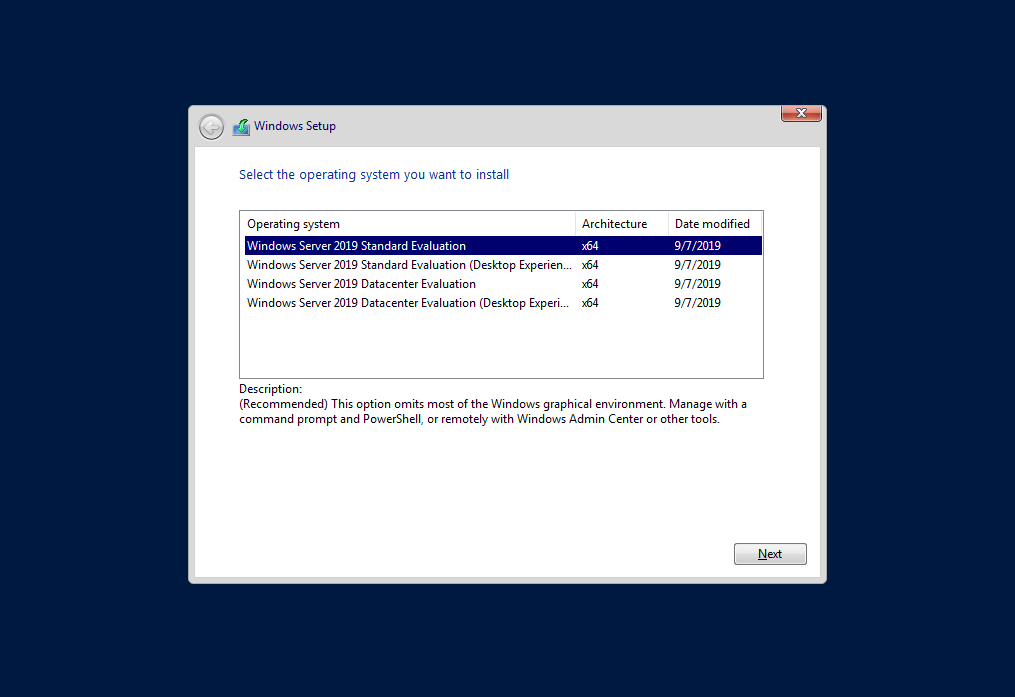
\includegraphics[width=0.5\textwidth]{Images/conf2en.PNG}
    \caption{Aggiunta dell'ISO}
\end{figure}



\subsubsection{GUI}
Qui ci basterà cliccare la versione nel nostro caso Windows Server 2019 Standard Evaluation e cliccare su \textbf{next}.Dopo di che ci chiederà di accettare i termini della licenza bisogna accettare e andare avanti. Ci caricherà una schermata dove che tipo di installazione si vuole eseguire. Noi sceglieremo Quella personalizzata, ci verrà chiesto su che disco la vogliamo installare e ci mostrerà solo un disco. Quindi senza fare niente ci basterà cliccare su \textbf{next}. Dopo aver cliccato avanti partirà l'installazione. 


\begin{figure}[h]
    \centering
    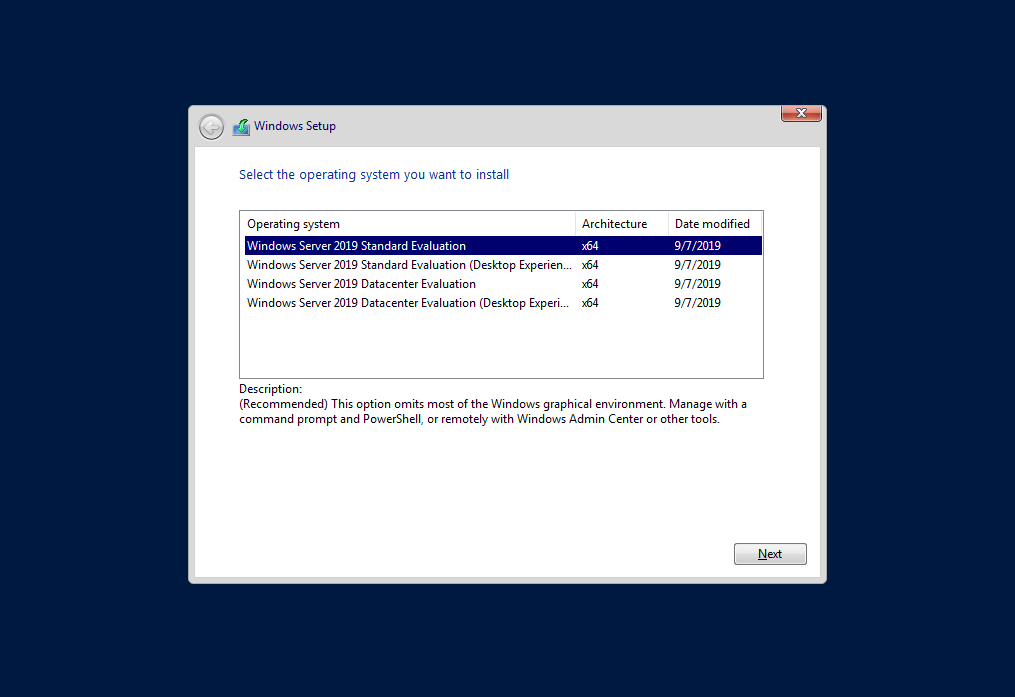
\includegraphics[width=0.5\textwidth]{Images/conf2en.PNG}
    \caption{Aggiunta dell'ISO}
\end{figure}


\subsubsection{Configurazione Core}
## Primi passi
Da qui ci dirà che la password verrà cambiata al primo login e quindi dopo aver cliccato invio ci chiederà la nuova password che andrà messa 2 volte e una volta fatto saremo dentro come amministratore.

## Cambiare il nome al server
Per cambiare il nome al nostro server dovremo digitare il comando "SConfig" e poi premere il numero 2. Ci verrà chiesto di inserire il nome del nostro server una volta fatto il sistema andrà riavviato.

\begin{figure}[h]
    \centering
    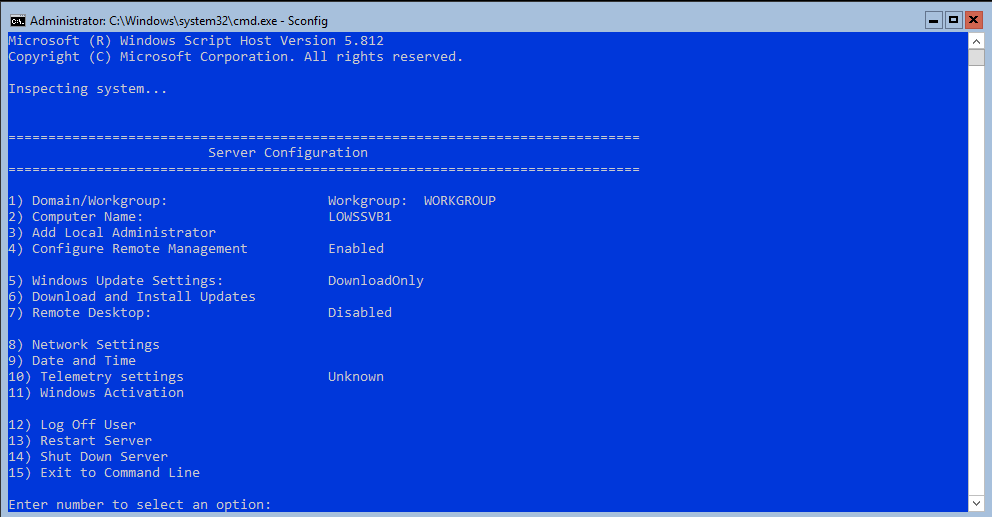
\includegraphics[width=0.5\textwidth]{Images/coreConf1.PNG}
    \caption{Aggiunta dell'ISO}
\end{figure}


\subsubsection{ Mettere il server in dominio}
Per cambiare il dominio della macchina dovremo digitare "SConfig" e poi premere il tasto numero 1 e dopo premere la D.

\begin{figure}[h]
    \centering
    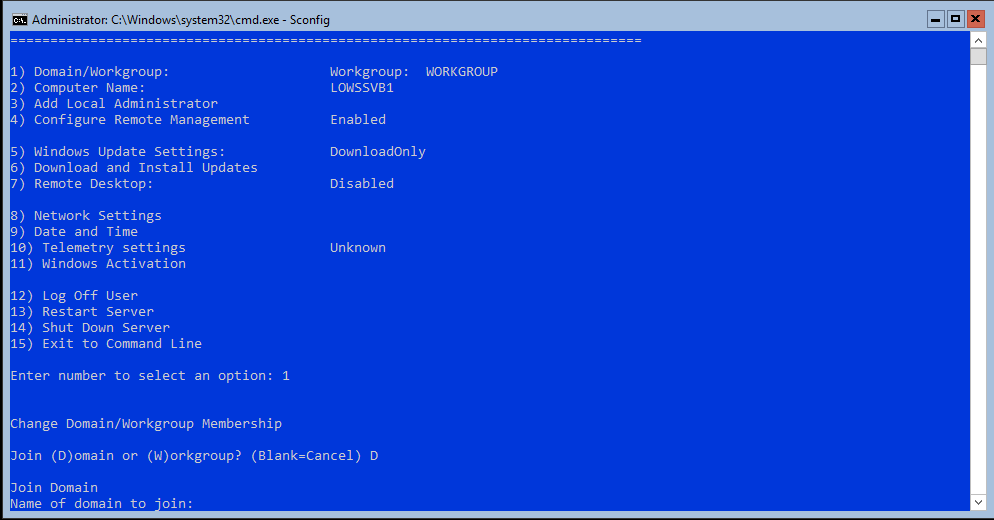
\includegraphics[width=0.5\textwidth]{Images/coreConf2.PNG}
    \caption{Aggiunta dell'ISO}
\end{figure}

Dopo aver digitato il nome del dominio/utente deve essere un utente autorizzato si ha anche la possibilità di modificare il nome del computer prima del riavvio. Poiché abbiamo già cambiato il nome del computer nel passaggio precedente, fare clic su No.



\subsubsection{Impostazione delle rete }
Per cambiare l’impostazione di rete dovremo digitare il comando "SConfig" e poi premere il tasto numero 8.

\begin{figure}[h]
    \centering
    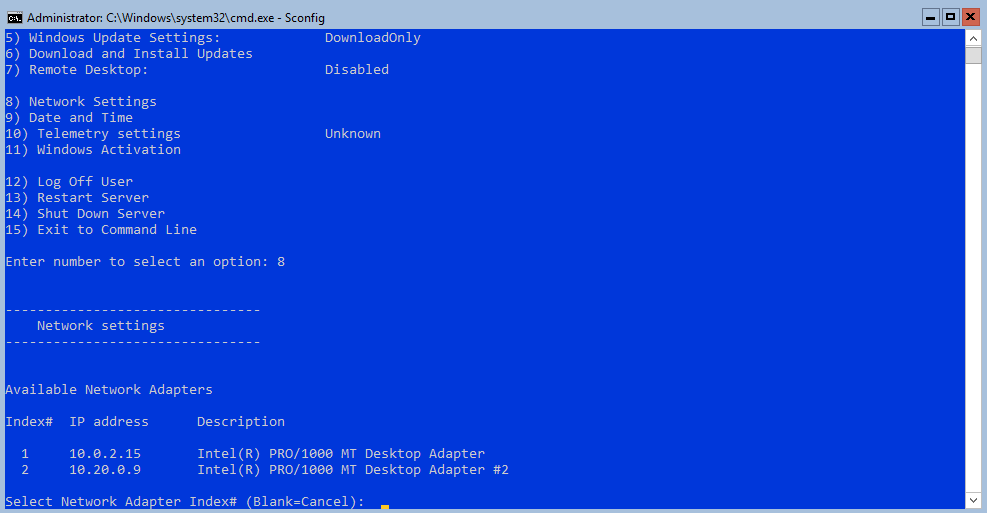
\includegraphics[width=0.5\textwidth]{Images/coreConf3.PNG}
    \caption{Aggiunta dell'ISO}
\end{figure}

Prima di tutto andiamo a digitare 1 cosi da modificare la rete NAT del nostro server. Una volta fatto ci basterà cliccare invio e ci porterà sulla prossima schermata.

\begin{figure}[h]
    \centering
    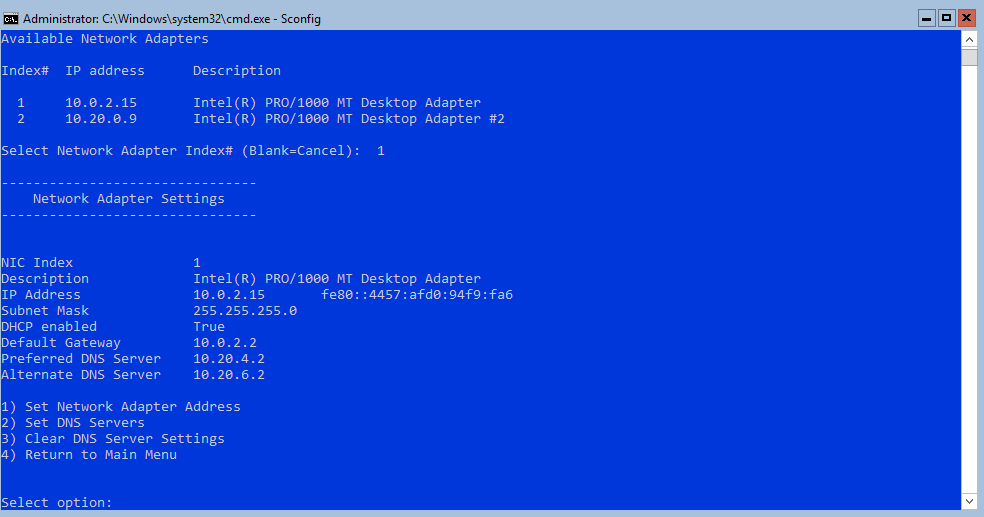
\includegraphics[width=0.5\textwidth]{Images/coreConf4.PNG}
    \caption{Aggiunta dell'ISO}
\end{figure}
Qui prima andiamo a digitare il numero 1 e poi premio s cosi da impostare un ip statico. Prima inseriamo l'ip che vogliamo dare alla macchina poi la subnet mask. Una volta fatto questo ci verrà chiesto anche il default gateway fatto anche quello ci basterà fare invio e avremmo assegnato al nostro server un ip statico. Dopo di andiamo a impostare il DNS ci basterà cliccare il numero 2. Una volta impostato potremmo tornare alla schermata di base premendo il tasto 4.


\textbf{In caso che si vuole anche impostare la seconda scheda di rete il processo é lo stesso.}

\end{document}  
